%#!platex ./report.tex

\chapter{$B7k2L(B}
 \section{Passive$B$N7k2L(B}
   \subsection{$B@h9T8&5f<jK!(B\cite{torben2009systematic}$B$H$NHf3S(B}
     $B@h9T8&5f$GMQ$$$i$l$F$$$?8DBNI>2A;XI8$H$NHf3S$r0J2<$N?^(B\ref{Tsuishi_Rerative}$B$K<($9(B. 
     \begin{figure}[H]
       \centering
       \hspace*{-1cm}
       \begin{subfigure}{0.4\columnwidth}
         \centering
         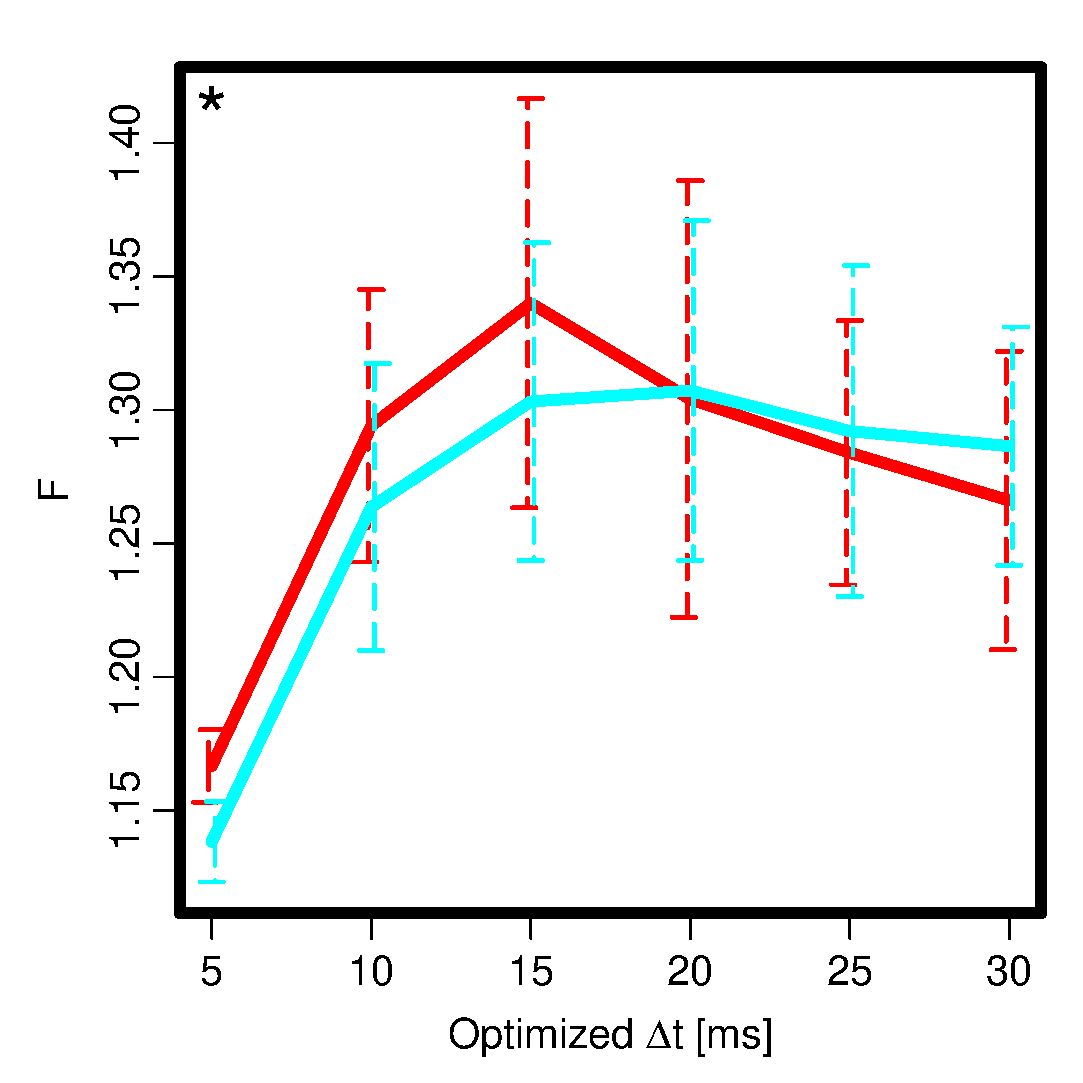
\includegraphics[width=\columnwidth]{./Images_Result/Tsuishi_Rerative_F.eps} 
         \caption{F$BCM(B}
         \label{Tsuishi_Rerative_F}
       \end{subfigure}
       \begin{subfigure}{0.4\columnwidth}
         \centering
         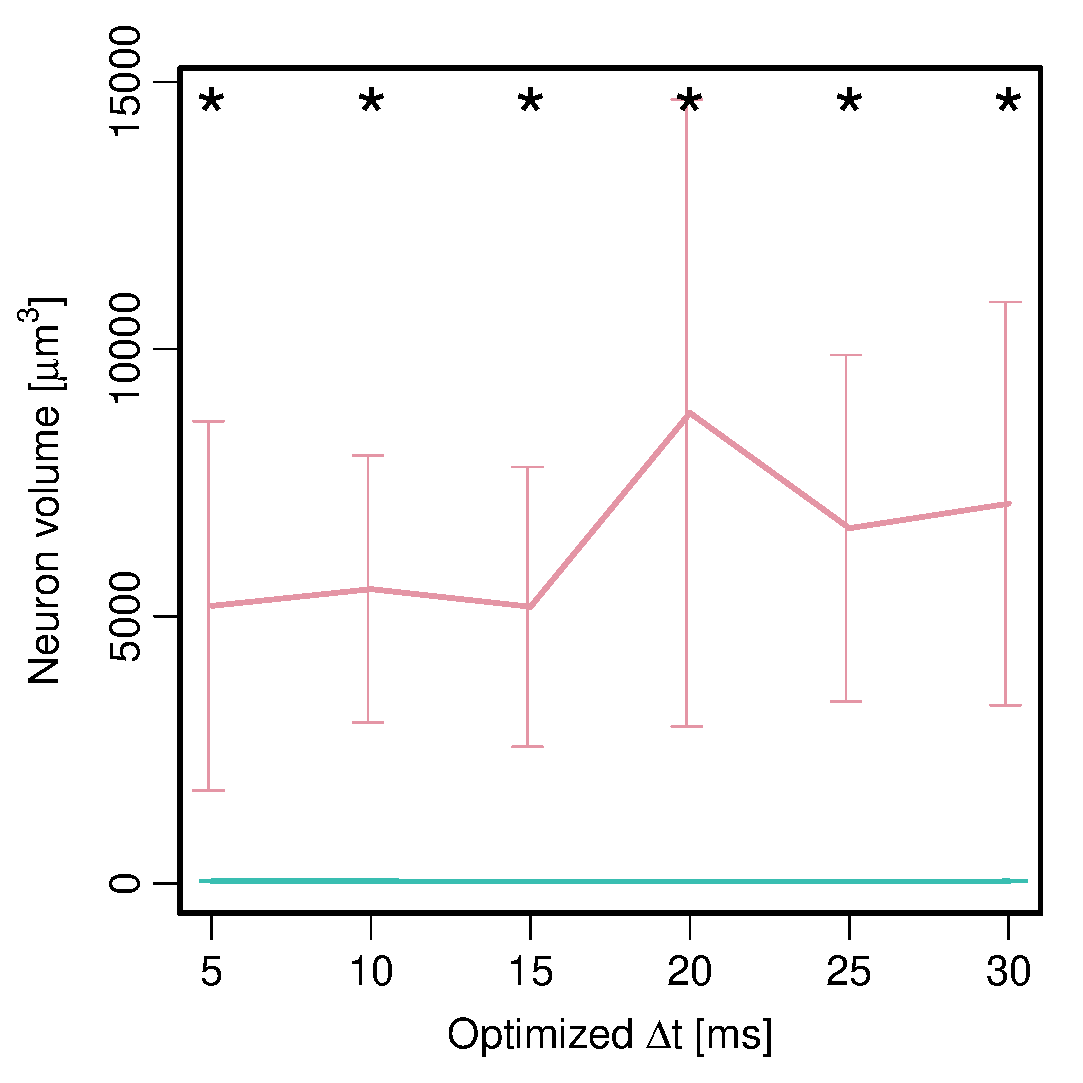
\includegraphics[width=\columnwidth]{./Images_Result/Tsuishi_Rerative_TREE_volume.eps} 
         \caption{$BBN@Q(B}
         \label{Tsuishi_Rerative_volume}
       \end{subfigure}

       \hspace*{-2.5cm}
       \begin{subfigure}{0.4\columnwidth}
         \centering
         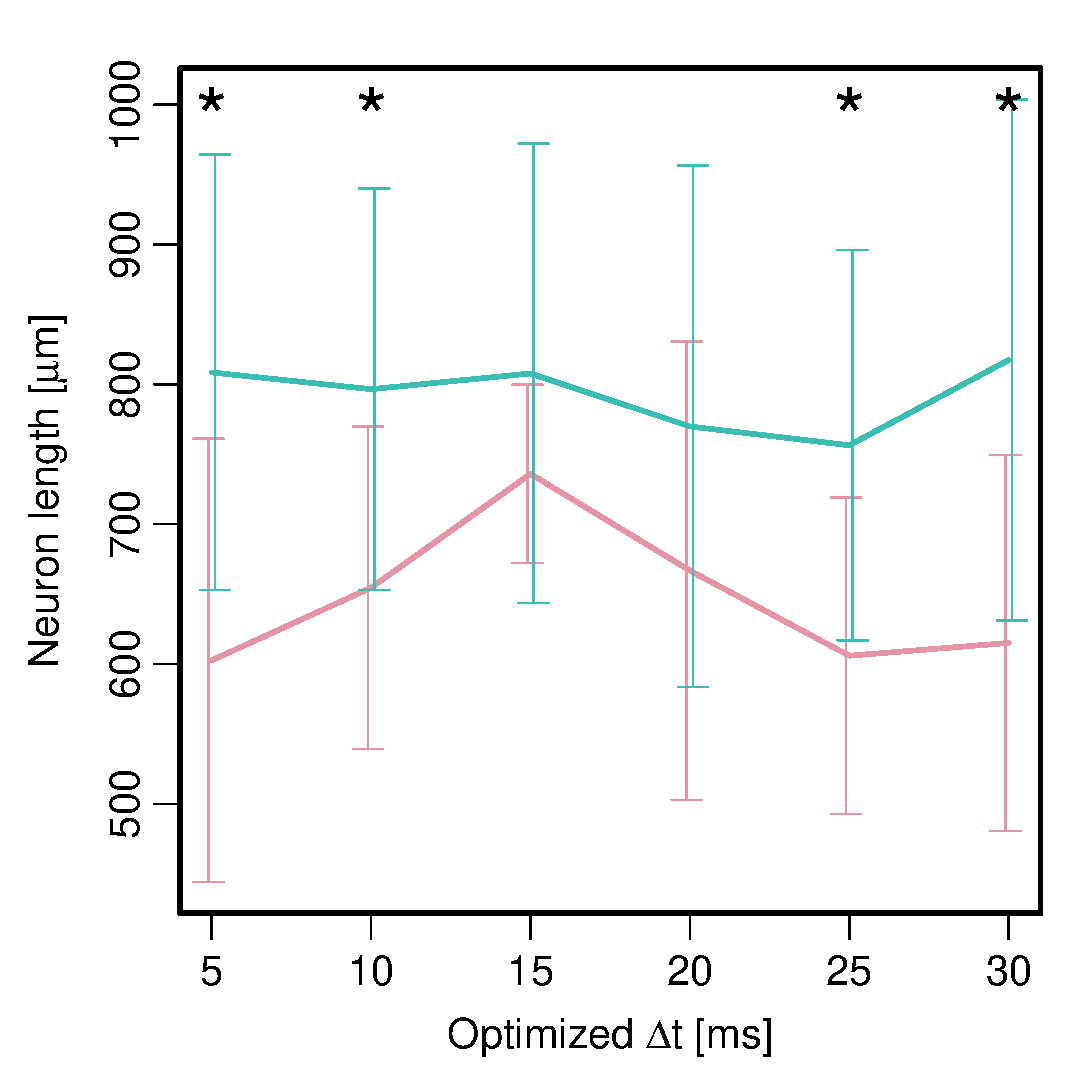
\includegraphics[width=\columnwidth]{./Images_Result/Tsuishi_Rerative_TREE_length.eps} 
         \caption{$BD9$5(B}
         \label{Tsuishi_Rerative_length}
       \end{subfigure}
       \begin{subfigure}{0.3\columnwidth}
         \centering
         \includegraphics[width=\columnwidth]{./Images_Result/Tsuishi_Rerative_legend.eps} 
       \end{subfigure}

     \caption{$B@h9T8&5f<jK!$H$NHf3S(B}
     \label{Tsuishi_Rerative}
   \end{figure}

     $B?^Cf$N9u$$@10u(B(${\star}$)$B$O(B, $B3F(B${\Delta}t$[ms]$B$K$*$$$F@h9T8&5f<jK!$rMQ$$$?>l9g(B
     (Torben et al)$B$HK\8&5f<jK!(B(Rerative)$B$N4V$G%9%A%e!<%G%s%H$N(Bt$B8!Dj(B(${\alpha} = 0.05$)$B$r(B
     $BMQ$$(B, $BM-0U:9$"$j$H$J$C$?$3$H$r<($9(B. % $B$3$l$"$C$F$s$N!)(B
     $B?^(B\ref{Tsuishi_Rerative_volume}$B$+$i$o$+$k$h$&$KK\8&5f$N<jK!$NJ}$,L@$i$+$KBN@Q$N(B
     $BBg$-$5$,>.$5$/$J$C$F$$$k(B. 
 \section{Ka$B%A%c%M%k$rMQ$$$?>l9g$N7k2L(B}
 \section{CaT$B%A%c%M%k$rMQ$$$?>l9g$N7k2L(B}
 \section{Ka$B%A%c%M%k(B, CaT$B%A%c%M%k$rMQ$$$?>l9g$N7k2L(B}

